\documentclass{beamer}
\begin{document}
\title{Hierarchical Path-Finding}
\author{Addie Audette, Bug Lee, Annorah Lewis, Luke Marks}
\date{December 12, 2022} 

\frame{\titlepage} 

\frame{\frametitle{Table of contents}\tableofcontents} 


\section{Path finding background} 
\frame{\frametitle{Path finding} 
You are given
\begin{itemize}
  \item Starting location $S$
  \item Destination location $D$
\end{itemize}

\begin{figure} 
\centering
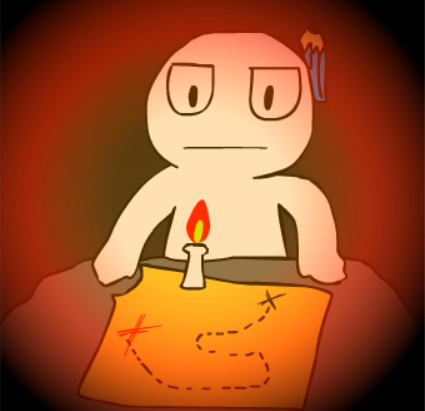
\includegraphics[scale=0.5]{imgs/path_finding.png}
\end{figure}
}

\frame{\frametitle{Path finding} 
You want to avoid path from $S$ to $D$ that are 
\begin{itemize}
  \item Impossible
  \item Dangerous
  \item Unnecessary
\end{itemize}

\begin{figure} 
\centering
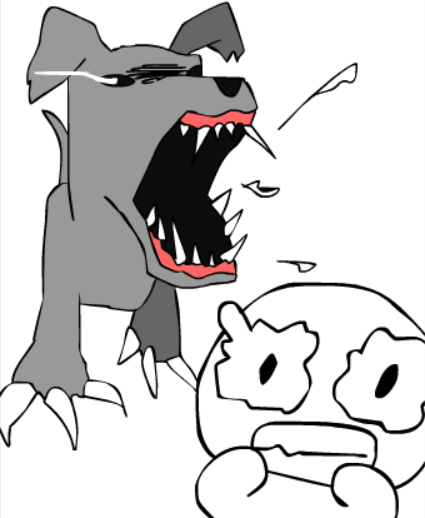
\includegraphics[scale=0.4]{imgs/dangerous_path.png}
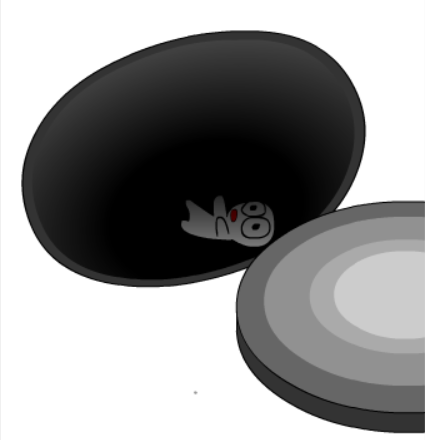
\includegraphics[scale=0.4]{imgs/wrong_path.png}
\end{figure}
}

\subsection{Grid graph}
\frame{\frametitle{Viewing world with grid graph} 
Imagine world is made of grid, like mindcraft...

\begin{figure} 
\centering
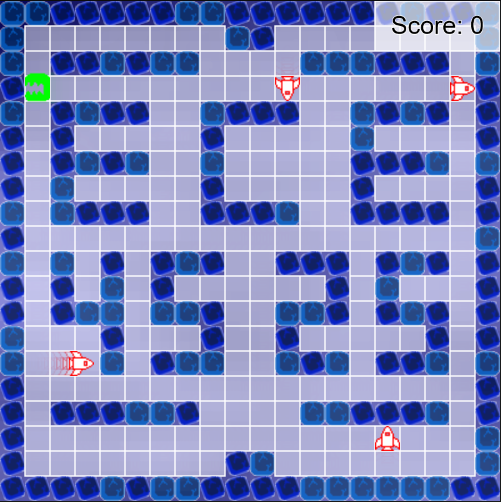
\includegraphics[scale=0.4]{imgs/grid_world.png}
\end{figure}
}

\frame{\frametitle{Viewing world with grid graph} 
Each vertex have degree 4 and edges are undirected with weight 1.

\begin{figure} 
\centering
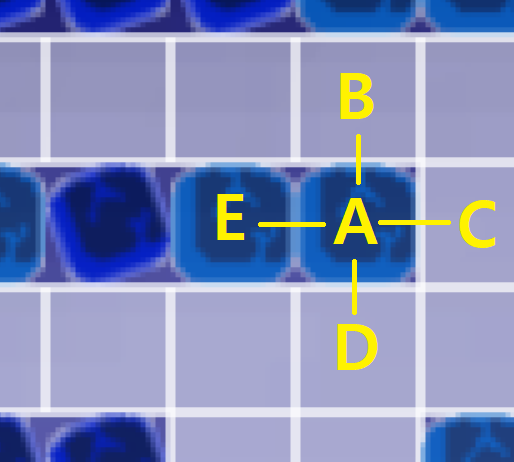
\includegraphics[scale=0.4]{imgs/adjacency.png}
\end{figure}
We will come back to the grid graph later...
}


\section{Shortest path algorithms}
\subsection{Dijkstra}
\frame{\frametitle{Dijkstra}
\begin{itemize}
  \item Dijkstra algorithm finds the shortest path to all the vertices from source $s$, given that the graph $G = (V, E)$ contains only non-negative weight for all edges\cite{CLRS}. 
  \item In other words, it forms the tree that represents the shortest paths to all of the vertices in the graph. 
\end{itemize}

\begin{figure} 
\centering
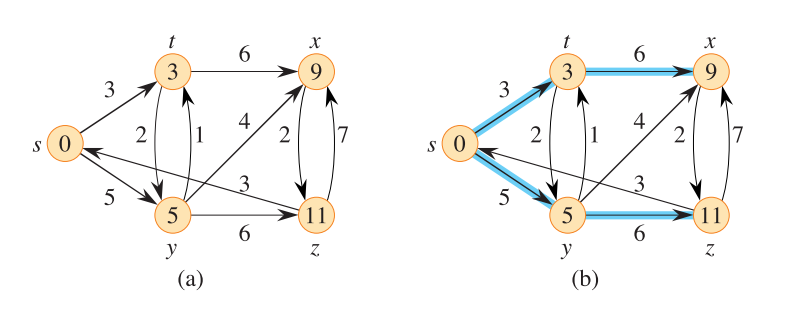
\includegraphics[scale=0.5]{imgs/shortest_path_tree.png}
\caption{(a) A weighted, directed graph with source $s$. (b) The blue edges represent the shortest-path tree rooted at the source $s$. The figure was taken from \textit{Introduction to Algorithms} by CLRS\cite{CLRS}.} 
\end{figure}

}

\subsection{A*}
\frame{\frametitle{A*}
\begin{itemize}
  \item "Dijkstra with a twist" \cite{Buckland}
  \item Dijkstra algorithm blindly selects vertex with minimum distance from $s$ each step. Instead, make a clever guess in each step where the algorithm selects a vertex that is likely part of the shortest path from $s$ to $t$.\cite{Buckland, HNR}
\end{itemize}
}
\frame{\frametitle{A*: Clever guess?}
For A* to work correctly and efficiently, the A* algorithm must guess each step that
\begin{itemize}
    \item Heuristic: \\
    Minimize unnecessary computation on finding sub-paths that are obviously not part of the optimal path\cite{HNR}, but also 
    \item Admissiblity: \\
    Should not ignore the sub-path that can be part of the optimal path\cite{HNR}.  
\end{itemize}
}

\subsection{Shortcomings}
\frame{\frametitle{Shortcomings}
In practice, a naive A* algorithm is still not sufficient for many modern applications. 
\begin{enumerate}
  \item Many modern applications require computation to happen in real-time for hundreds, if not thousands, users/agents simultaneously\cite{Botea2004NearOH}.
  \item The shift to mobile applications has put more limitations on memory and CPU usage\cite{Botea2004NearOH}.
\end{enumerate}
}

\section{Hierarchical Path Finding}
\subsection{Using hierarchy to reduce complexity}
\frame{\frametitle{Using hierarchy to reduce compleixty}
The idea of Hierarchical Path Finding is to form a region by clustering the vertices and introducing high-level regional routes. 
\begin{enumerate}
  \item Compute a local (low-level) route to the source to the source region entrance, 
  \item Compute a regional (high-level) route from the source region to destination region, and 
  \item Compute a local (low-level) route to destination region exit to destination.
\end{enumerate}

\begin{figure} 
\centering
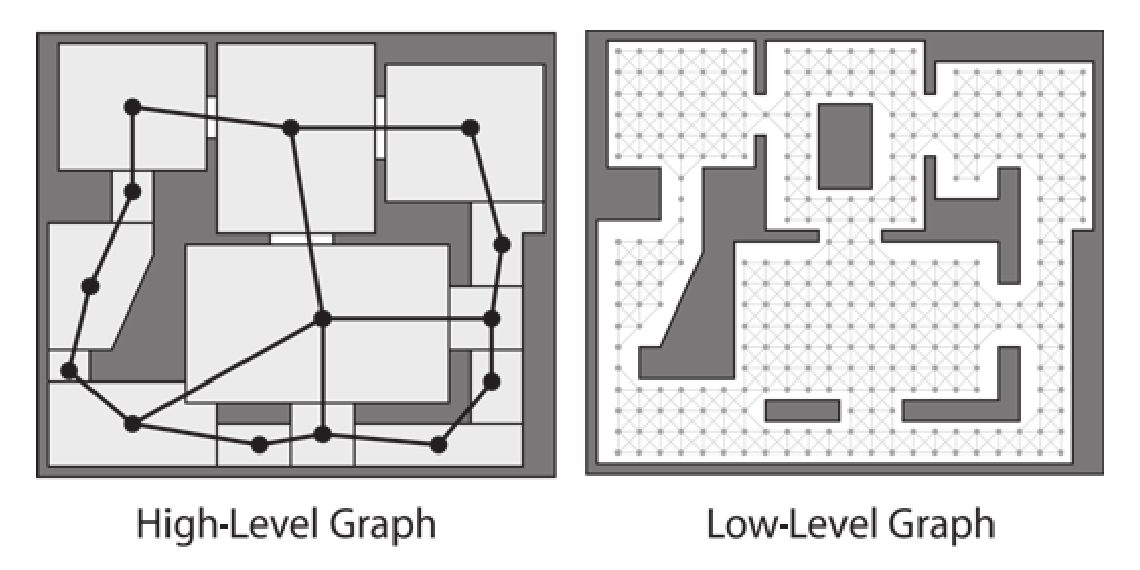
\includegraphics[scale=0.2]{imgs/hierarchy.png}
\caption{Forming regions (high-level graph) by clustering neighboring vertices. The figure was taken from \textit{Programming Game AI by Example} by Buckland\cite{Buckland}.} 
\end{figure}
}

\subsection{Challenges}
\frame{\frametitle{Challenges}
Compare to Dijkstra and naive A*, there are more tunable variables that implementers need to consider
\begin{itemize}
  \item The number of hierarchy levels, 
  \item Cluster/region size, and 
  \item Placement of regional entrances/exits. 
  \item In practice, optimizations like preprocessing/caching regional routes and path smoothing may be necessary.
\end{itemize}
}
\frame{\frametitle{Simplification}
To avoid overwhelming the algorithm with optimization details, our implementation assume the following simplifications: 
\begin{enumerate}
  \item An input graph is static and known in advance, 
  \item 2 level of the hierarchy, 
  \item Randomly distributes regional entrances/exits in reachable locations, 
  \item No preprocessing/caching, and 
  \item No path refinement or smoothing.
\end{enumerate}
}

\subsection{Experiment results}
\frame{\frametitle{Experiment setup}
\begin{figure} 
\centering
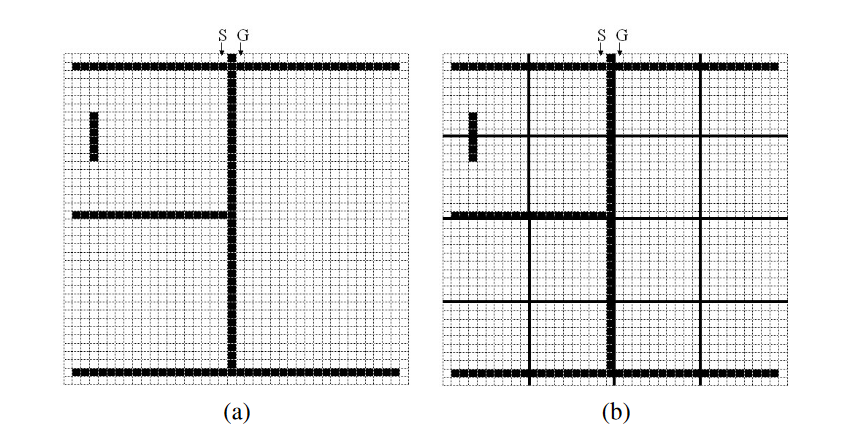
\includegraphics[scale=0.5]{imgs/experiment_setup.png}
\caption{(a) The 40 X 40 maze used in our example. The obstacles are painted in black. $S$ and $G$ are the start and the goal nodes. (b) The bold lines show the boundaries of the 10x 10 clusters\cite{Botea2004NearOH}.} 
\end{figure}
}
\frame{\frametitle{Experiment results}
\begin{center}
\begin{tabular}{| c | c | c |}
    \hline
    Algorithm & \# of vertices visited & Time (ms) \\
    \hline
    Dijkstra & 0 & 0 \\
    A* & 0 & 0 \\
    Hierarchical Path Finding & 0 & 0 \\
    \hline
\end{tabular}
\end{center}
** We are still working on experimentation. We hope to provide experiment results during revision.
}


\section{Limitations}
\subsection{Near optimal path}
\frame{\frametitle{Limitations}
\begin{itemize}
  \item Hierarchical Path Finding does not guarantee the shortest path between the source and destination. 
  \item The \textit{Near Optimal Hierarchical Path-Finding} apply a path-smoothing procedure to make a path found by Hierarchical Path Finding within $1\%$ optimal compared to shortest path\cite{Botea2004NearOH}.
\end{itemize}
}

\frame{\frametitle{References}
\bibliographystyle{plain}
\bibliography{references.bib}
}

\end{document}